\section{Durchführung}
\label{sec:Durchführung}

\subsection{Magnetfeld von Spulen}
\begin{figure}
    \caption{Hallsonde und Spule \cite{anleitung1}.}
    \centering
    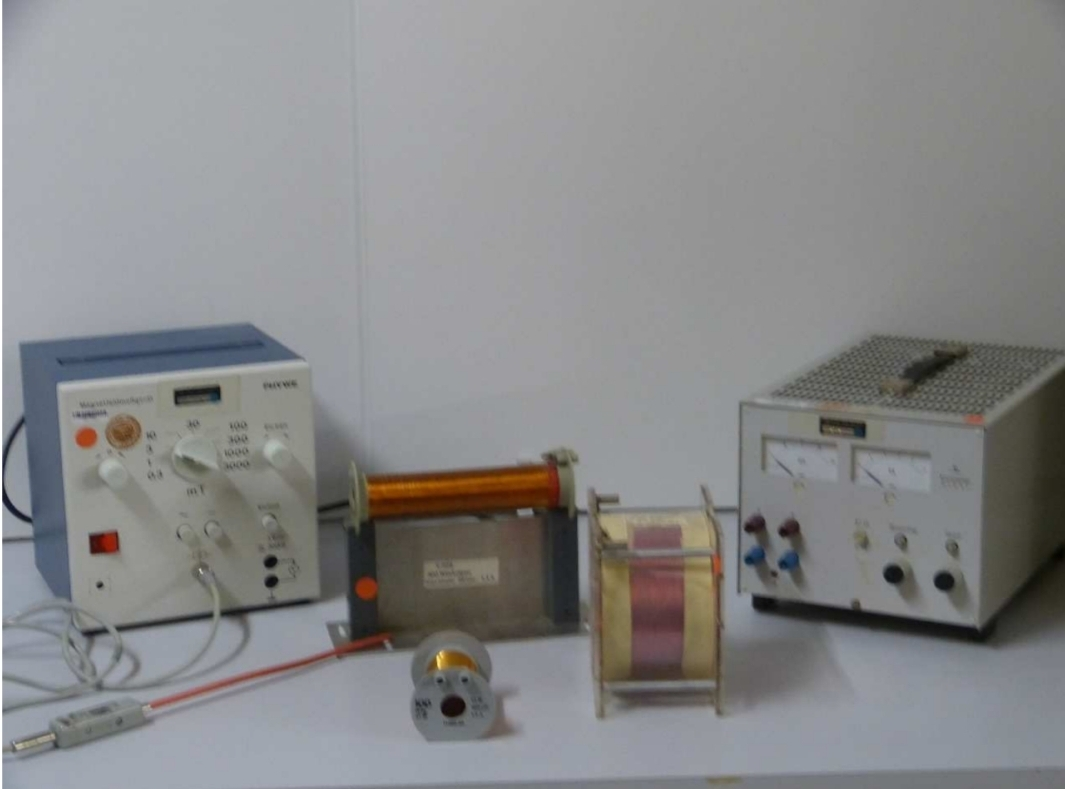
\includegraphics[width=0.7\textwidth]{"Bilder/mvs.jpg"}
\end{figure}
\noindent Der Versuchsaufbau ist recht simpel, zwei Spulen (eine längere, welche
von beiden Seiten untersucht werden muss und eine kürzere) werden untersucht,
dazu werden eine Hall-Sonde (befestigt auf einem Lineal) und ein Steuergerät
verwendet.

Die im Bild zu erkennende Spule wird mithilfe einer longitudinalen Hall-Sonde 
untersucht, diese wird dazu langsam in die Spule eingeführt. Jeweils in 1 cm-
Abständen wird die Magnetfeldstärke gemessen und dokumentiert, außerhalb der 
Spule werden bereits Messwerte aufgenommen. Der Strom wird maximal aufgedreht 
für den Strom wird 1 A angelegt. Es ist darauf 
zu achten, dass das alles möglichst präzise platziert wird; die Hall-Sonde auf 
dem Lineal, die Spule parallel zu diesem, sowie die Ausrichtung der Sonde bei 
Einführung in die Spule. Da das Magnetfeld nicht überall identisch ist, können 
bereits kleine Abweichungen zu unterschiedlichen Ergebnissen bei der Dokumentation 
der Magnetfeldstärke führen. 

Dieser Vorgang wird für eine längere und eine kürzere Spule durchgeführt. Bei 
der kürzeren reicht es, die Hall-Sonde von einer Seite durchzuführen. Die andere 
Spule hingegen ist jedoch zu lang, sodass die Sonde beidseitig hineingeleitet 
wird.

\subsection{Hysteresekurve}
\begin{figure}
    \caption{Toroidspule mit Eisenkern \cite{anleitung1}.}
    \centering
    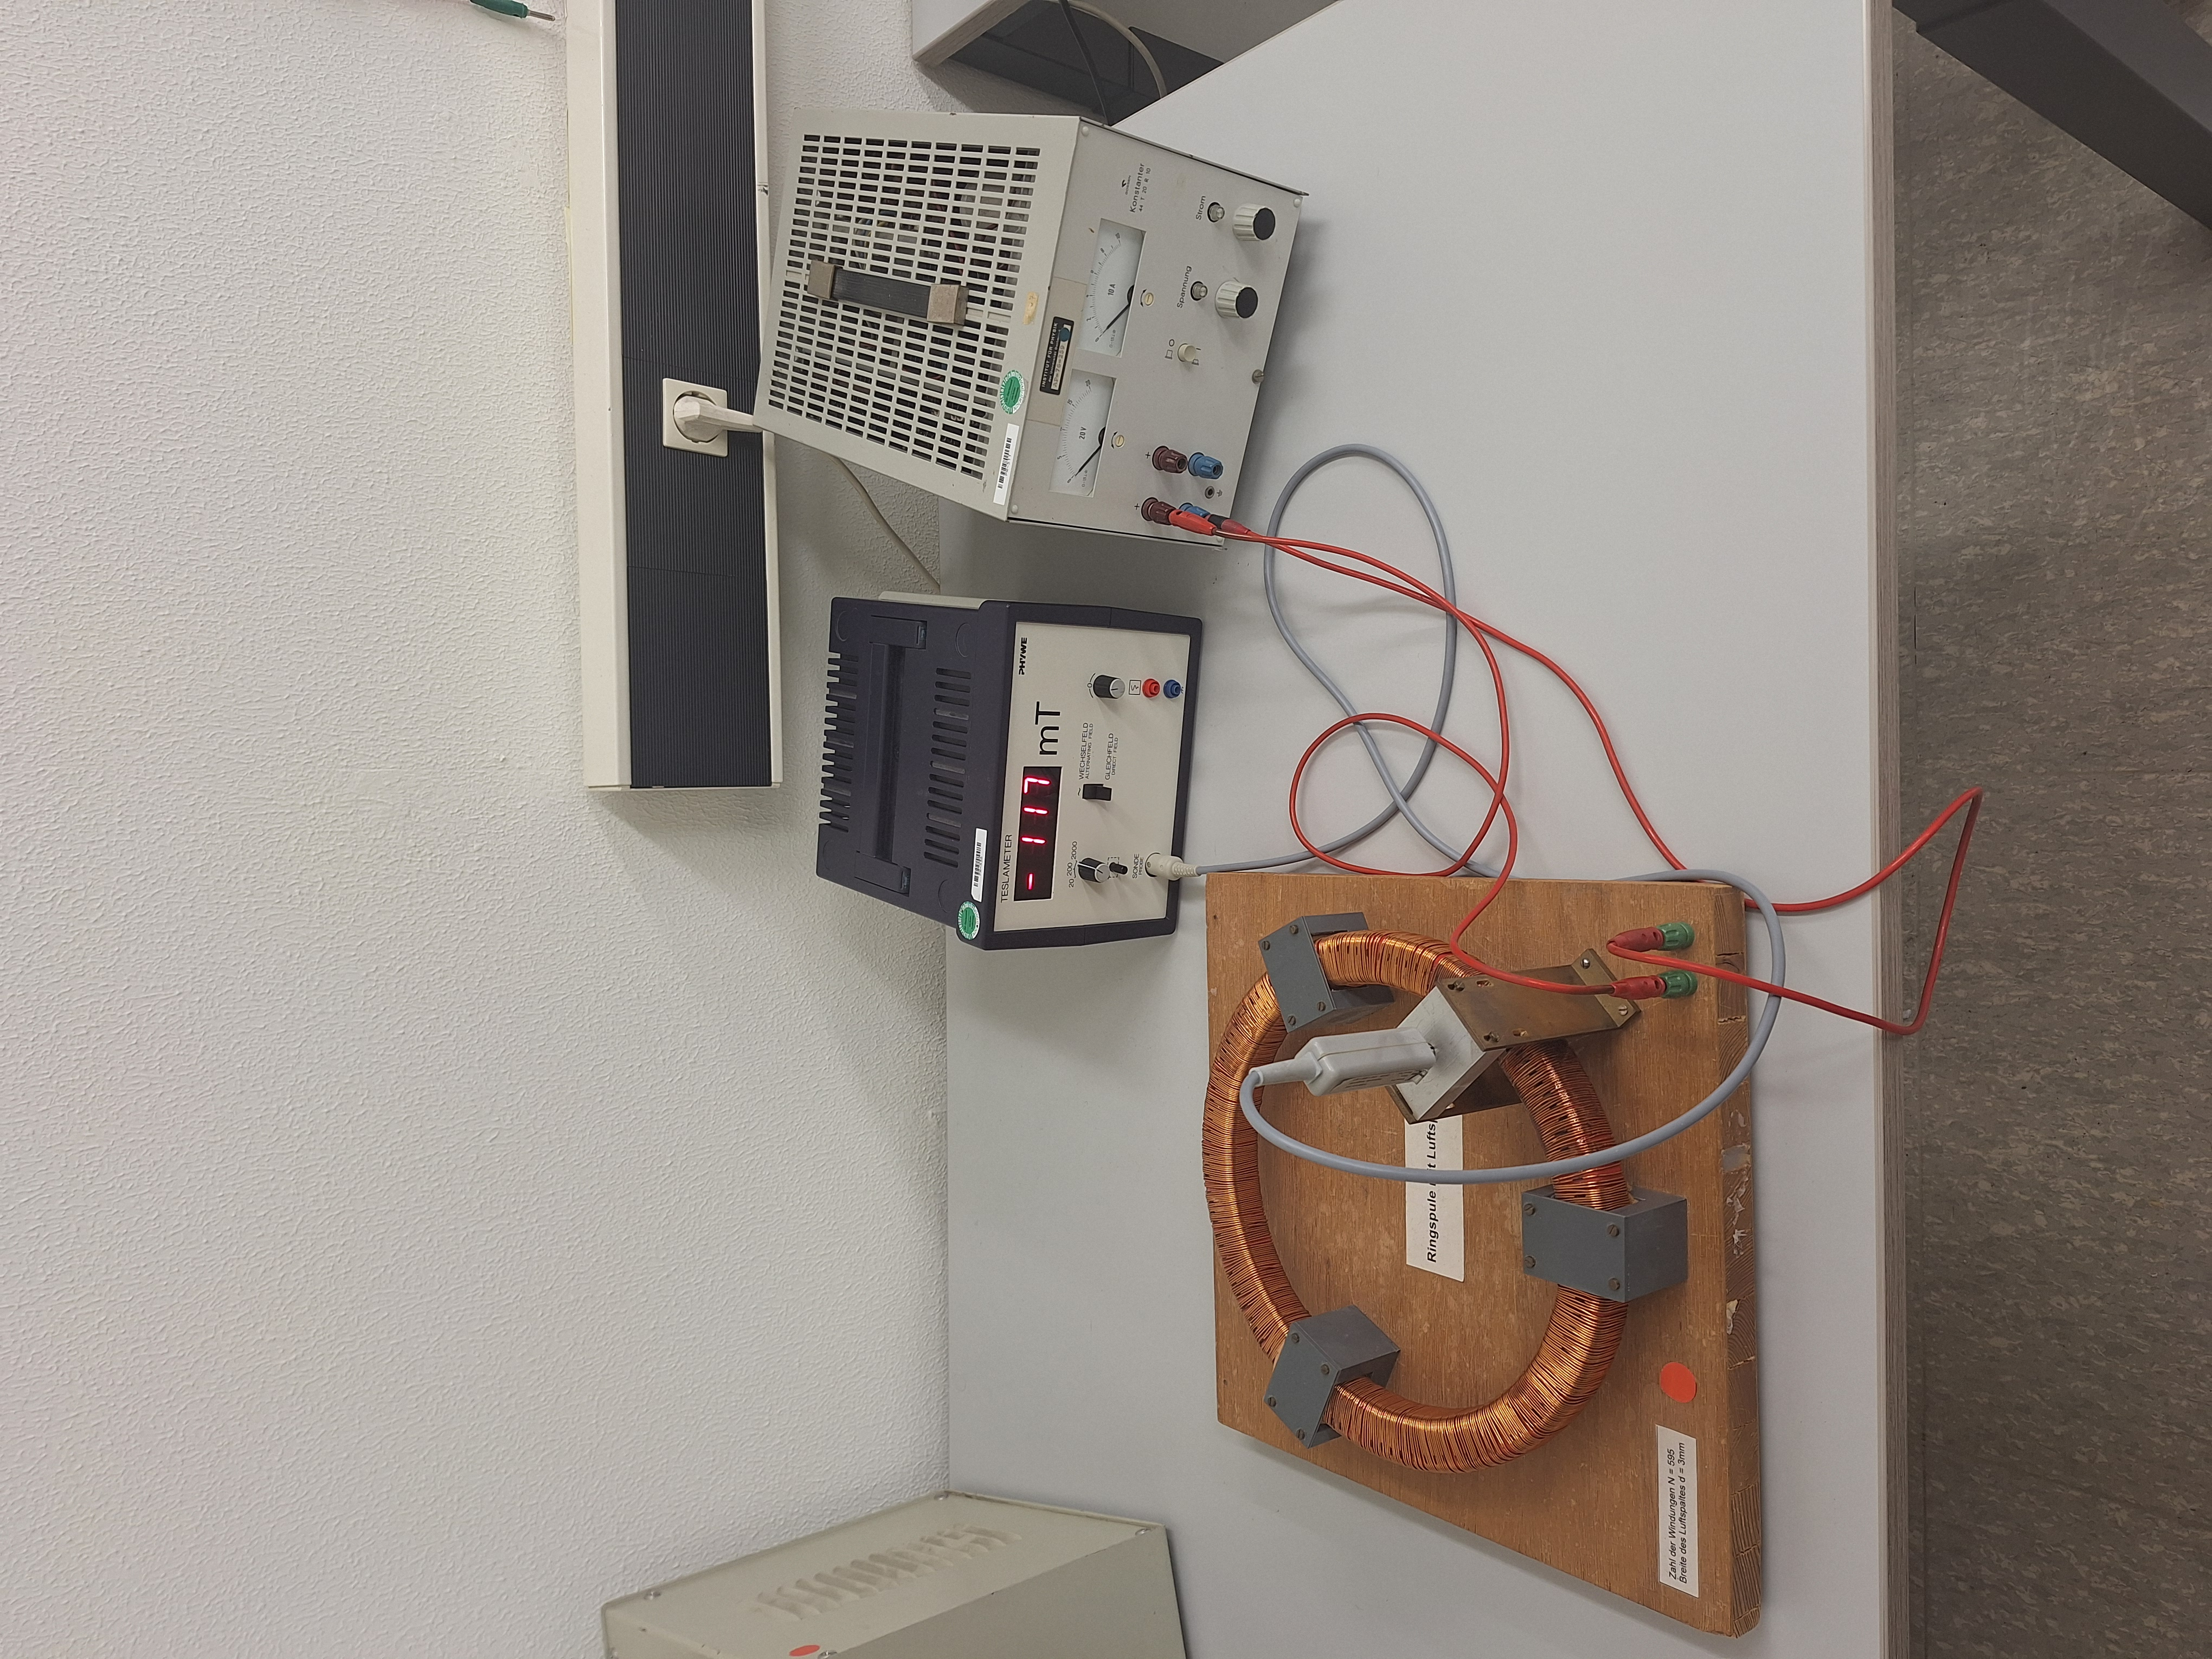
\includegraphics[width=0.7\textwidth, angle=-90]{"Bilder/hysterese.jpg"}
\end{figure}
\noindent Der Versuchsaufbau unterscheidet sich nicht wesentlich von dem Vorherigen, 
es liegt eine Ringspule mit Luftspalt vor, welche an ein Netzgerät und eine 
transversale Hall-Sonde angeschlossen ist. Genau so wird eine maximale Spannung 
angelegt. Wichtig ist, dass eine Entmagnetisierung der Torusspule stattfindet, 
damit kein Magnetfeld das Experiment beeinflusst.
Um nun an die gefragte Hysteresekurve, Sättigungsmagnetisierung, Remanenz 
und Koerzitivkraft zu gelangen, wird der Strom variiert; Es wird eine Steigerung 
um 1 A bis zu einem Limit von 5 A gewählt. Der höchste Wert gibt schlussendlich
den Sättigungswert $B_S$ an. Darauffolgend wird der Strom in identischen 
Abständen wieder herunterreguliert. Wird kein Spulenstrom mehr detektiert, so 
kann an der Hall-Sonde die Remenanz abgemessen werden. Anschließend findet eine 
Umpolung statt, welche möglichst schnell stattfinden sollte, damit ungewünschte 
Effekte wie Energieverluste oder thermische Effekte vermieden werden können. 
Weiterhin wird die Stromstärke wie gehabt schrittweise erhöht (bis zur negativen 
Sättigung $B_S$) und danach wieder verringert, woraufhin eine letzte Umpolung 
stattfindet und der Versuch anschließend beendet wird.

\subsection{Helholtz-Spule}
\begin{figure}
    \caption{Spulenpaar \cite{anleitung1}.}
    \centering
    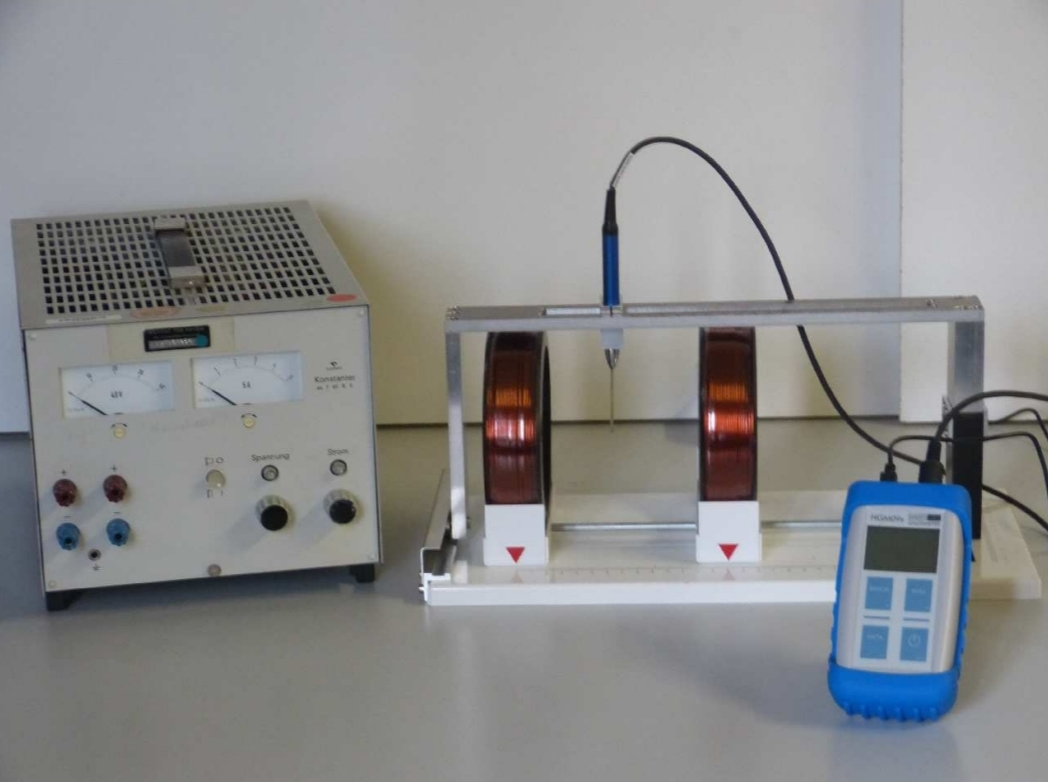
\includegraphics[width=0.7\textwidth]{"Bilder/helmholtz.jpg"}
\end{figure}
\noindent Das in der Abbildung gezeigte Helmholtz-Spulen-Paar wird in Reihe 
geschaltet bei einer maximalen Spannung. Die Spulen werden zunächst in einem
beliebigen Abstand ausgerichtet, mithilfe der transversalen Hall-Sonde wird
dann die Magnetfeldstärke in 1 cm-Abständen gemessen, jenes geschieht sowohl
innerhalb-als auch außerhalb der Spule. Bei dem Messvorgang wird eine Stromstärke 
von 5 A nicht überschritten. Die gemessenen Ergebnisse werden dann
mit den theoretischen Werten verglichen.